\chapter{Progettazione e codifica}
\label{cap:progettazione-codifica}

\intro{Breve introduzione al capitolo}\\

\section{Tecnologie e strumenti}
\label{sec:tecnologie-strumenti}

Di seguito viene data una panoramica delle tecnologie e strumenti presi in considerazione per lo sviluppo del prototipo.

\subsection{Strumenti analizzati}
Durante le prime due settimane di Stage è stato condotto uno studio preliminare su diversi strumenti di security testing per AI generativa. Di seguito viene fornita la matrice di valutazione dei tools e una breve descrizione di ciascuno strumento analizzato.

\begin{figure}[!h]
    \centering
    % includegraphics is redefined in config/thesis-config.tex to prepend
    % the images/ folder, so here we only pass the filename
    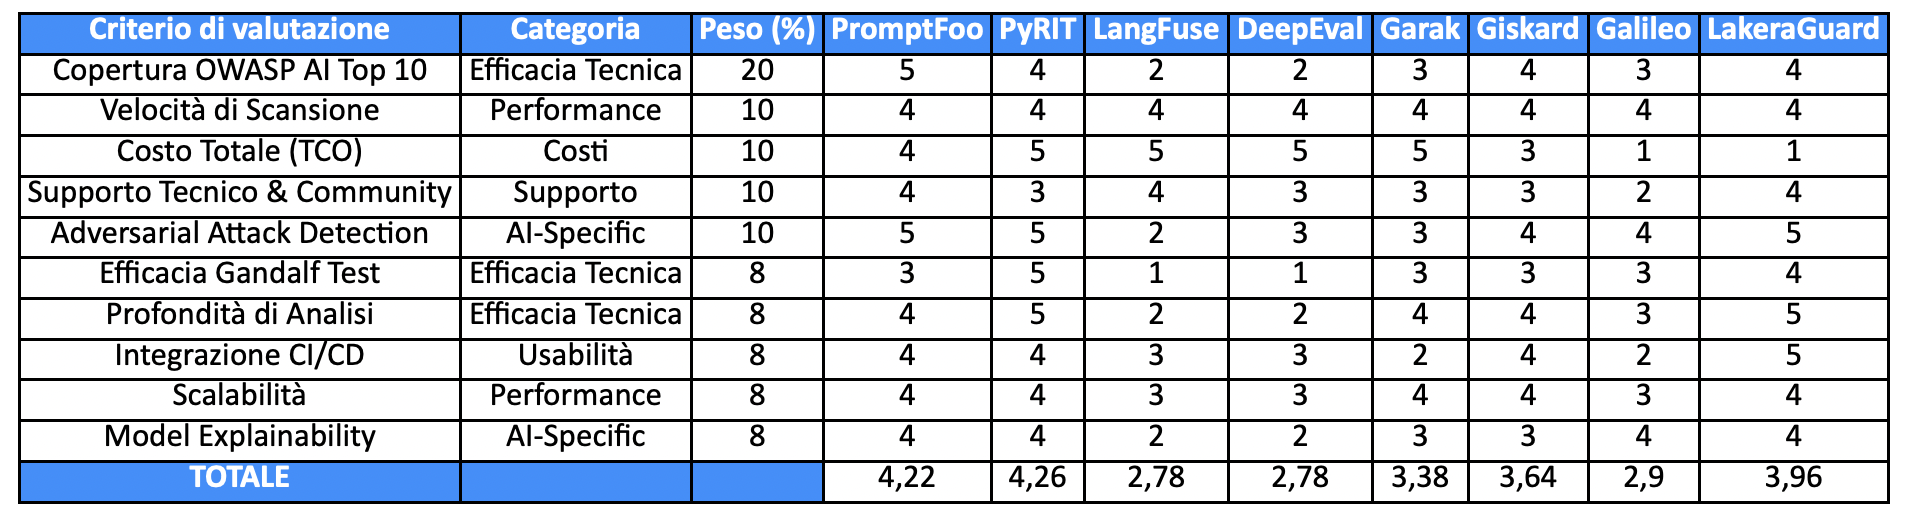
\includegraphics[width=1.0\columnwidth]{matrix.png}
    \caption{Matrice di Valutazione degli Strumenti Analizzati}
\end{figure}

\subsubsection*{PromptFoo}
PromptFoo è una piattaforma di testing per modelli di linguaggio che consente agli sviluppatori di creare, eseguire e gestire test automatizzati per valutare le prestazioni, l'affidabilità e la sicurezza dei loro modelli di linguaggio naturale (NLP). Offre funzionalità come la creazione di casi di test personalizzati, l'integrazione con pipeline CI/CD e report dettagliati sui risultati dei test.
Questo tool è stato tenuto in molta considerazione in quanto offre funzionalità specifiche per il testing delle vulnerabilità OWASP top 10 per AI generativa, obbiettivo principale del progetto di stage.

\subsubsection*{PyRIT}
PyRIT è uno tool open-source progettato da Azure Microsoft per l'identificazione e la mitigazione dei rischi associati all'uso di modelli di intelligenza artificiale generativa. PyRIT è stato creato per valutare modelli di AI per potenziali vulnerabilità di sicurezza, bias e problemi di conformità, fornendo raccomandazioni su come migliorare la sicurezza e l'affidabilità dei modelli.\\
PyRIT è il tool su cui si è basato lo sviluppo del prototipo per la sua estensiva documentazione, per la sua facilità di utilizzo e per le sue molteplici funzionalità.

\subsubsection*{LangFuse}
LangFuse

\subsubsection*{DeepEval}
DeepEval è un framework open-source per la valutazione e il benchmarking dei modelli di intelligenza artificiale generativa. DeepEval non fornisce funzionalità specifiche per il testing dei modelli, per ovviare a questo è stato creato un tool di testing basato su DeepEval chiamato DeepTeam, un tool di red teaming, che però non ha un focus sulle vulnerabilità OWASP in quanto si concentra sul testing delle safety guidelines.

\subsubsection*{Garak}
Garak è uno scanner di vulnerabilità per modelli di intelligenza artificiale generativa open-source creato da NVIDIA per facilitare il testing dei modelli. Il focus di Garak sta nei metodi di attacco specifici per far fallire in modo imprevisto una LLM o un sistema di dialogo. Garak testa diverse vulnerabilità tra cui allucinazioni, data leakage, prompt injection, jailbreaks etc...

\subsubsection*{Giskard}
Giskard è una piattaforma di red teaming automatizzato per testare, valutare ed analizzare modelli di intelligenza artificiale generativa. Esistono due metodi di utilizzo di Giskard: Come servizio HUB a pagamento o come libreria python open-source da installare localmente. La libreria fornita è però fortemente limitata nelle funzionalità rispetto al servizio HUB in quanto incentrata sulla ricerca. Dopo una analisi approfondita del servizio HUB e dei costi associati è stato ritenuto incompatibile con gli obbiettivi del progetto di stage.

\subsubsection*{Galileo}
Galileo 

\subsubsection*{LakeraGuard}
LakeraGuard è una piattaforma di sicurezza per modelli di intelligenza artificiale che aiuta gli sviluppatori a proteggere i loro modelli da minacce e vulnerabilità. Offre funzionalità come la scansione delle vulnerabilità, la gestione delle patch e il monitoraggio delle minacce in tempo reale.\\
Il tool out of the box fà già quello che lo Stage chiede di implementare quindi non ha suscitato uno studio approfondito in quanto avrebbe reso superfluo lo sviluppo del prototipo.\\
Inoltre è un tool a pagamento che offre un tier gratuito il quale è però limitato a 10000 richieste \gls{api} al mese, limite che avrebbe reso difficile l'utilizzo futuro del tool.


\subsection{Strumenti scelti}
Di seguito viene data una panoramica delle tecnologie e strumenti utilizzati.


\section{Ciclo di vita del software}
\label{sec:ciclo-vita-software}

\section{Progettazione}
\label{sec:progettazione}

\subsubsection{Namespace 1} %**************************
Descrizione namespace 1.

\begin{namespacedesc}
    \classdesc{Classe 1}{Descrizione classe 1}
    \classdesc{Classe 2}{Descrizione classe 2}
\end{namespacedesc}


\section{Design Pattern utilizzati}

\section{Codifica}
